\chapter{Examples} \label{chap:examples}
The pruning algorithm is presented on several examples, where each of them has its purpose of being shown. The XOR problem (\cref{sec:dataset_xor}) should verify the ability of finding an optimal network structure. Section \ref{sec:dataset_unbfea} comes with another 2D problem, where one feature carries more information than the other one. The Rule-plus-Exception problem in \cref{sec:dataset_rpe} deals with a minority of samples that has to be treated by a different net part than rule-based samples. The train problem (\cref{sec:dataset_train}) is a working example of feature selection procedure. The MNIST database (\cref{sec:dataset_mnist}) is widely used in machine learning and can be regarded as commonly known. Therefore it is a good example for presentation of new methods. Finally, in \cref{sec:dataset_phonemes} the pruning algorithm is applied on a large dataset of phonemes.

\section{2D-problem: XOR Function} \label{sec:dataset_xor}
The standard Exclusive OR (XOR) function is defined by truth \cref{tab:examples:xor_function}. Based on this function one can build a classification problem with two features and two classes.

\begin{table}[H]
\centering
\begin{tabular}{|c|c||c|}
\hline
\textit{$ x_1 $} & \textit{$ x_2 $} & \textit{y} \\ \hline \hline
0                & 0                & 0          \\ \hline
0                & 1                & 1          \\ \hline
1                & 0                & 1          \\ \hline
1                & 1                & 0          \\ \hline
\end{tabular}
\caption{XOR function.}
\label{tab:examples:xor_function}
\end{table}

This problem serves perfectly for demonstration of network optimization methods, as two optimal architectural solutions producing the XOR function are known (\cref{fig:examples:xor_solutions}) \footnote{The known (e.g. from \citep{online:xor_solution}) minimal network architectures producing the XOR function $ [2, 2, 1] $ and $ [2, 3, 1] $ are adjusted to $ [2, 2, 2] $ and $ [2, 3, 2] $ in \cref{fig:examples:xor_solutions} in order to comply with the conventions introduced in \cref{chap:methods}. The number of output neurons always equals the number of classes. The number of synapses connected to the output layer is a subject to think about.}. 

\begin{figure}[H]
\centering
\begin{subfigure}{.4\textwidth}
  \centering
  \includegraphics[height=2cm]{xor_min1}
  \caption{Solution A.}
  \label{fig:examples:xor_min1}
\end{subfigure}
\begin{subfigure}{.4\textwidth}
  \centering
  \includegraphics[height=2cm]{xor_min2}
  \caption{Solution B.}
  \label{fig:examples:xor_min2}
\end{subfigure}
\caption{Optimal network architectures producing the XOR function.}
\label{fig:examples:xor_solutions}
\end{figure}

With this knowledge we can prove that the pruning algorithm is (or is not) able to find the optimal solution. If the method is correct, it should end up with one of the shown architectures (\cref{fig:examples:xor_min1} or \cref{fig:examples:xor_min2}).

The truth \cref{tab:examples:xor_function} ruled the generation of a 2D dataset illustrated in \cref{fig:examples:dataset_xor}. The two classes can be linearly separated by two lines (two neurons, see \cref{fig:examples:xor_min1}) and each class consists of 1000 samples. Each sample was randomly assigned to one of the two possible points belonging to its class (e.g. (0,0) or (1,1) for class 0) and then randomly placed in the surounding area within a specified range ($ r = \frac{\sqrt{2}}{4} $).

The samples of each class were then splitted into three sets in the following manner: $ 80\% $ to a training set, $ 10\% $ to a validation set and $ 10\% $ to a testing set.

\begin{figure}[H]
\centering
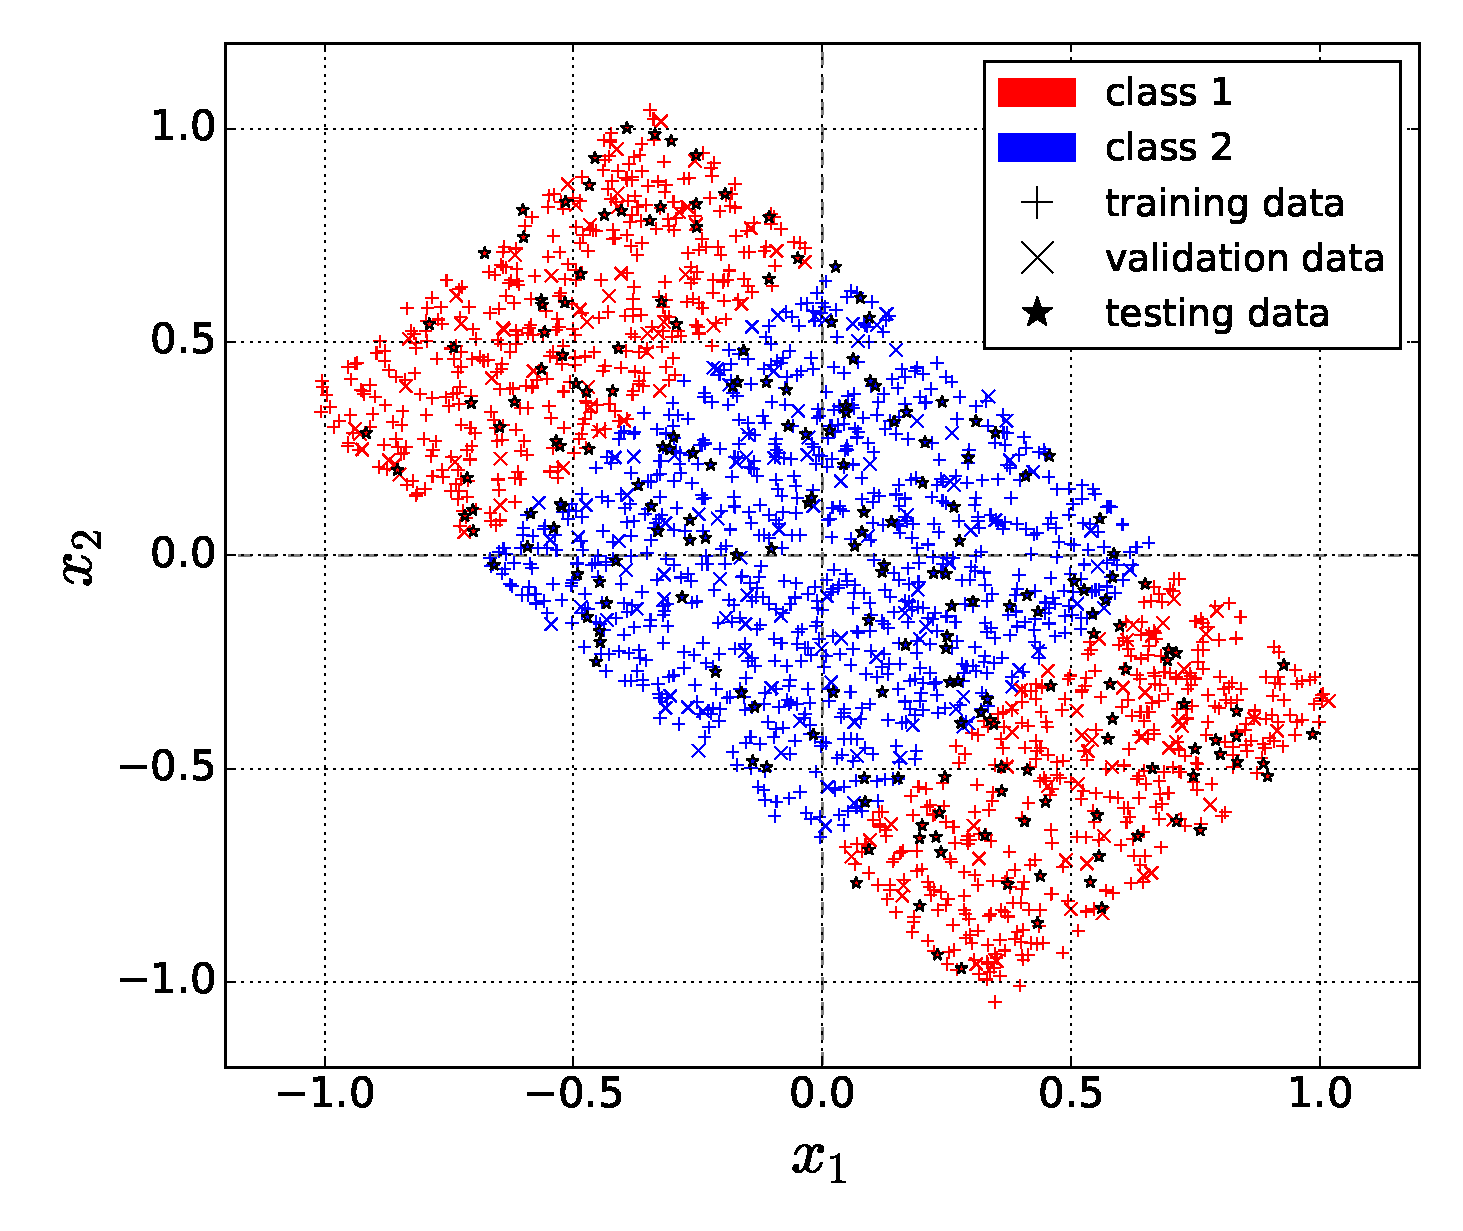
\includegraphics[width=0.9\textwidth]{dataset_xor.eps}
\caption{The XOR dataset.}
\label{fig:examples:dataset_xor}
\end{figure}

The goal of this example is to show that the pruning algorithm finds one of the known minimal network structures (\cref{fig:examples:xor_solutions}). An oversized network $ [2, 50, 2] $ is used as the starting point. The following \cref{tab:examples:xor_settings} shows all the experiment settings.

\begin{table}[H]
\centering
\scalebox{0.95}{
\begin{tabular}{|l|c|l|c|l|c|}
\hline
\multicolumn{2}{|c|}{\textit{initial network}} & \multicolumn{2}{c|}{\textit{learning parameters}} & \multicolumn{2}{c|}{\textit{pruning parameters}} \\ \hline
structure             & {[}2, 50, 2{]}         & learning rate                  & 0.3              & required accuracy             & 1.0              \\ \hline
transfer fcn          & sigmoid                & number of epochs               & 50               & retrain                       & True             \\ \hline
                      &                        & minibatch size                 & 1                & retraining epochs             & 50               \\ \hline
\end{tabular}}
\caption{Experiment settings for XOR dataset.}
\label{tab:examples:xor_settings}
\end{table}

\subsection*{Results: XOR Function}
\cref{fig:examples:pruning_process_xor} describes the pruning process. We can see the number of synapses (starting with $ 200 $ for fully-connected structure $ [2, 50, 2] $), the network structure and classification accuracy at single pruning steps (see [PA]). When the required accuracy ($ 1.0 $) was not reached, the corresponding steps are transparent in the figure, indicating they were forgotten.

\begin{figure}[H]
\centering
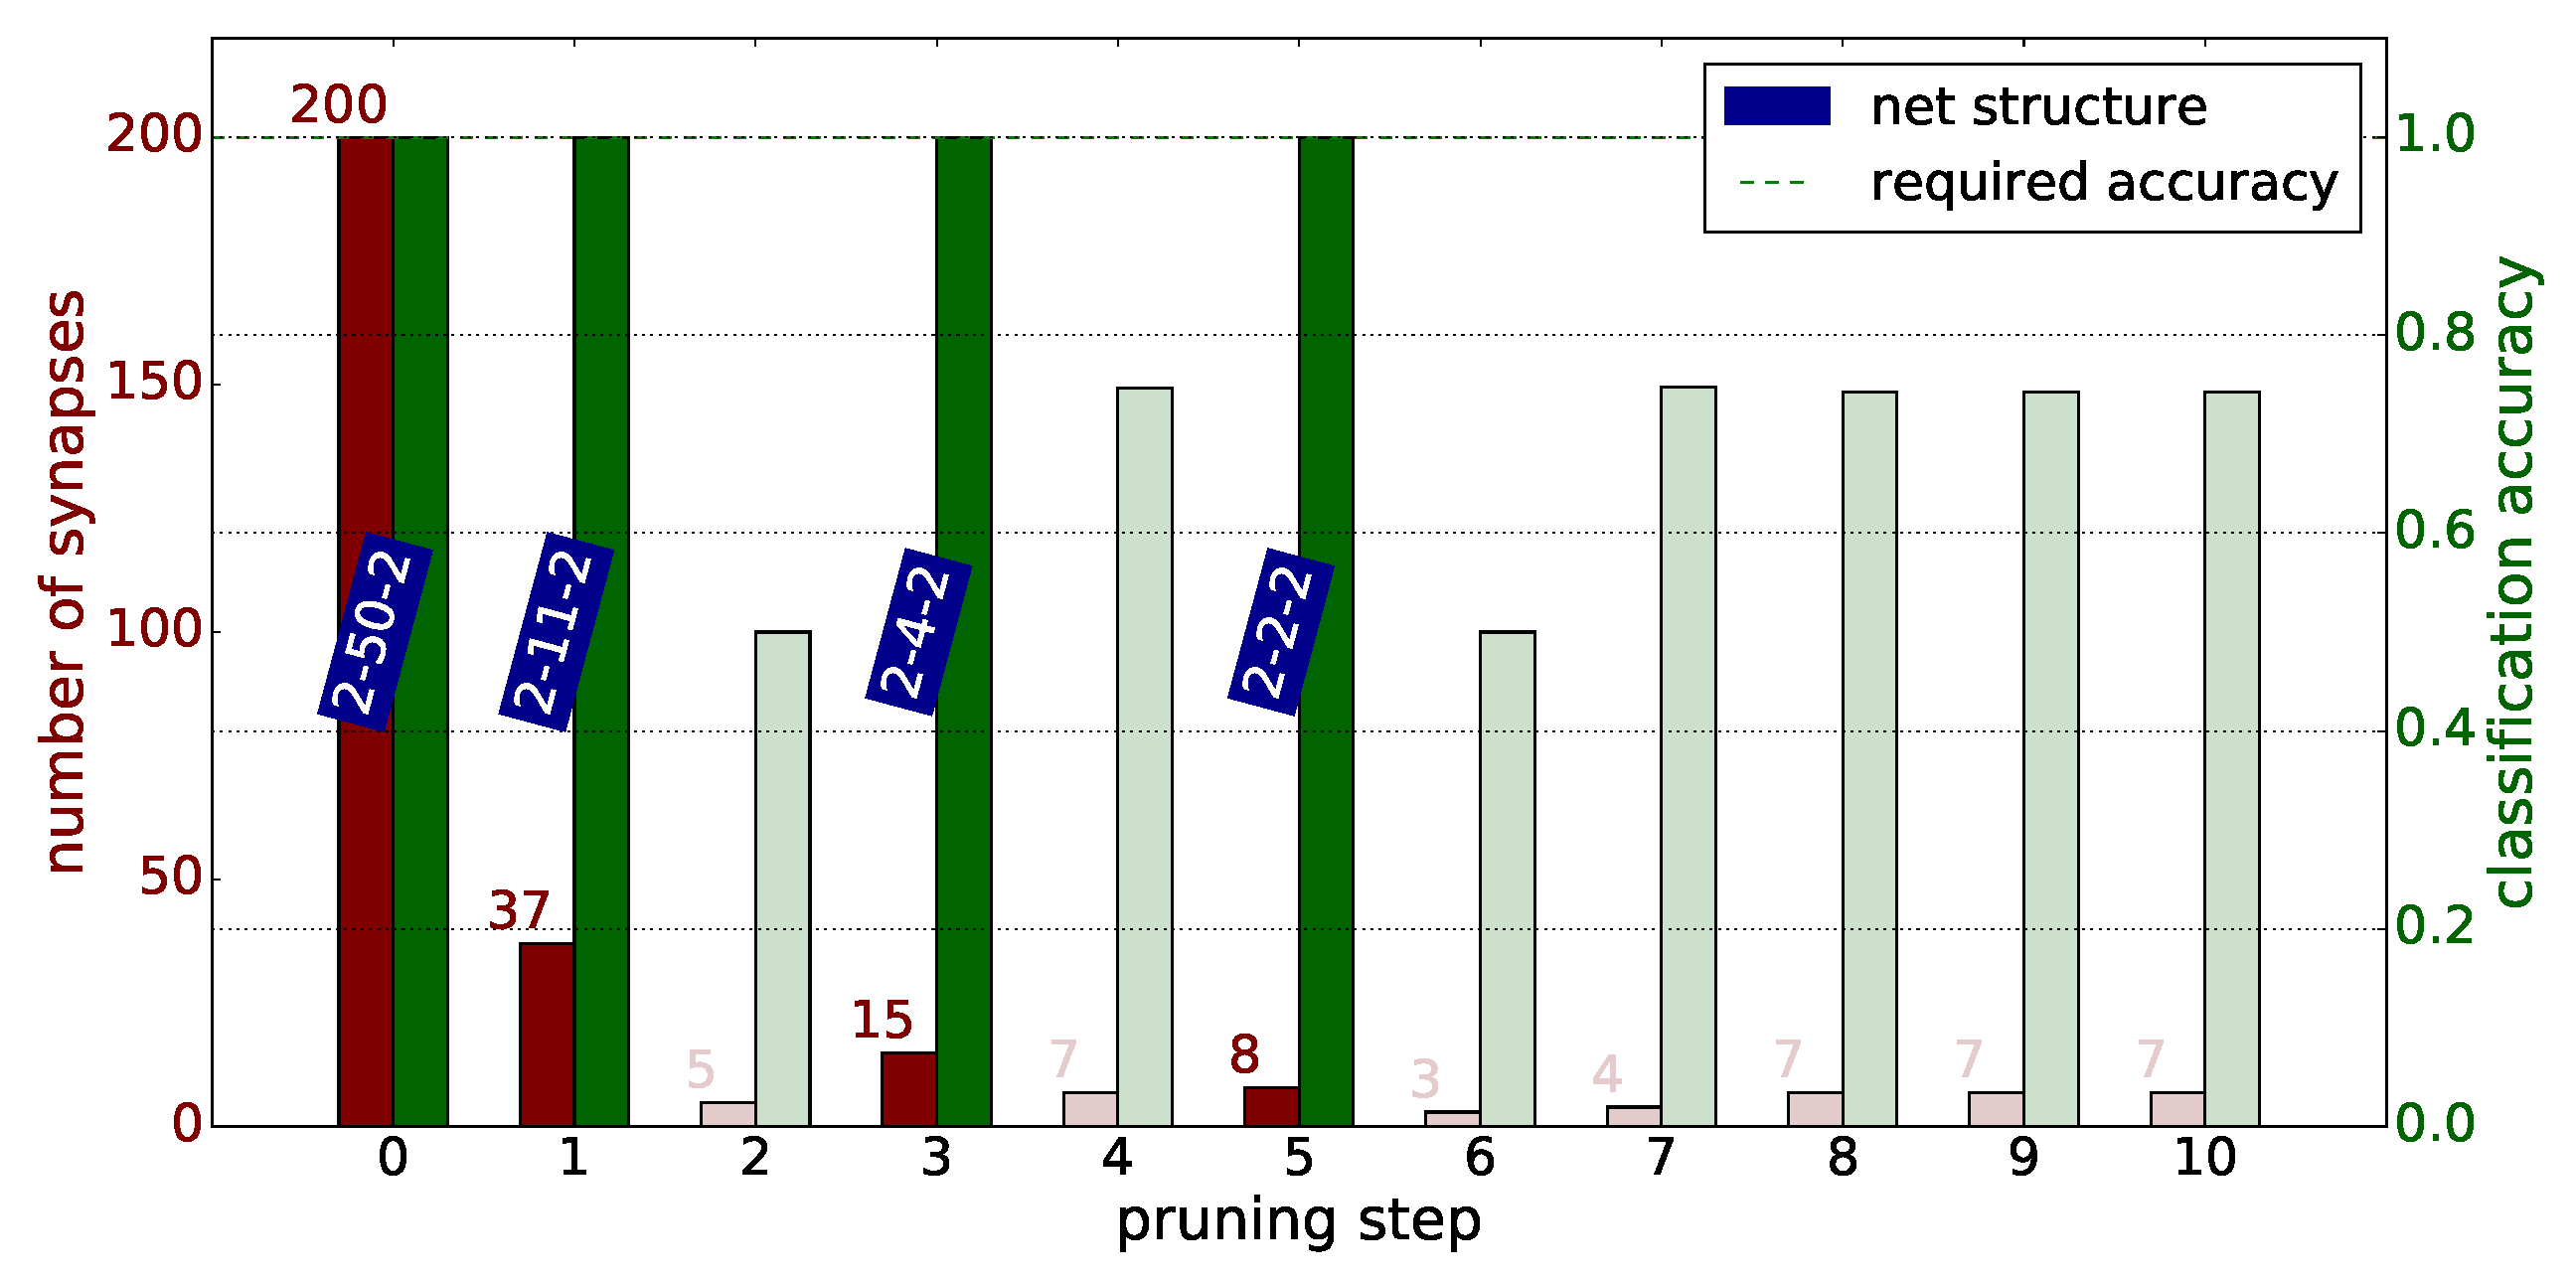
\includegraphics[width=\textwidth]{pruning_process_xor.eps}
\caption{Illustration of the pruning procedure applied on XOR dataset (selected observation).}
\label{fig:examples:pruning_process_xor}
\end{figure}

In \cref{fig:examples:pruning_result_xor} the hypothesis of this experiment is confirmed. In \cref{fig:examples:pie_xor} we can see that in $ 47 $ out of $ 100 $ cases the pruning algorithm changed the network to $ [2, 2, 2] $ architecture (\cref{fig:examples:xor_min1}), in $ 45\% $ of the cases it resulted with $ [2, 3, 2] $ (\cref{fig:examples:xor_min2}) and only in $ 8\% $ it failed to find the optimal architecture. \cref{fig:examples:result_synapses_xor} gives statistics for the final number of synapses in these three cases.

\begin{figure}[H]
\centering
\begin{subfigure}{.4\textwidth}
  \centering
  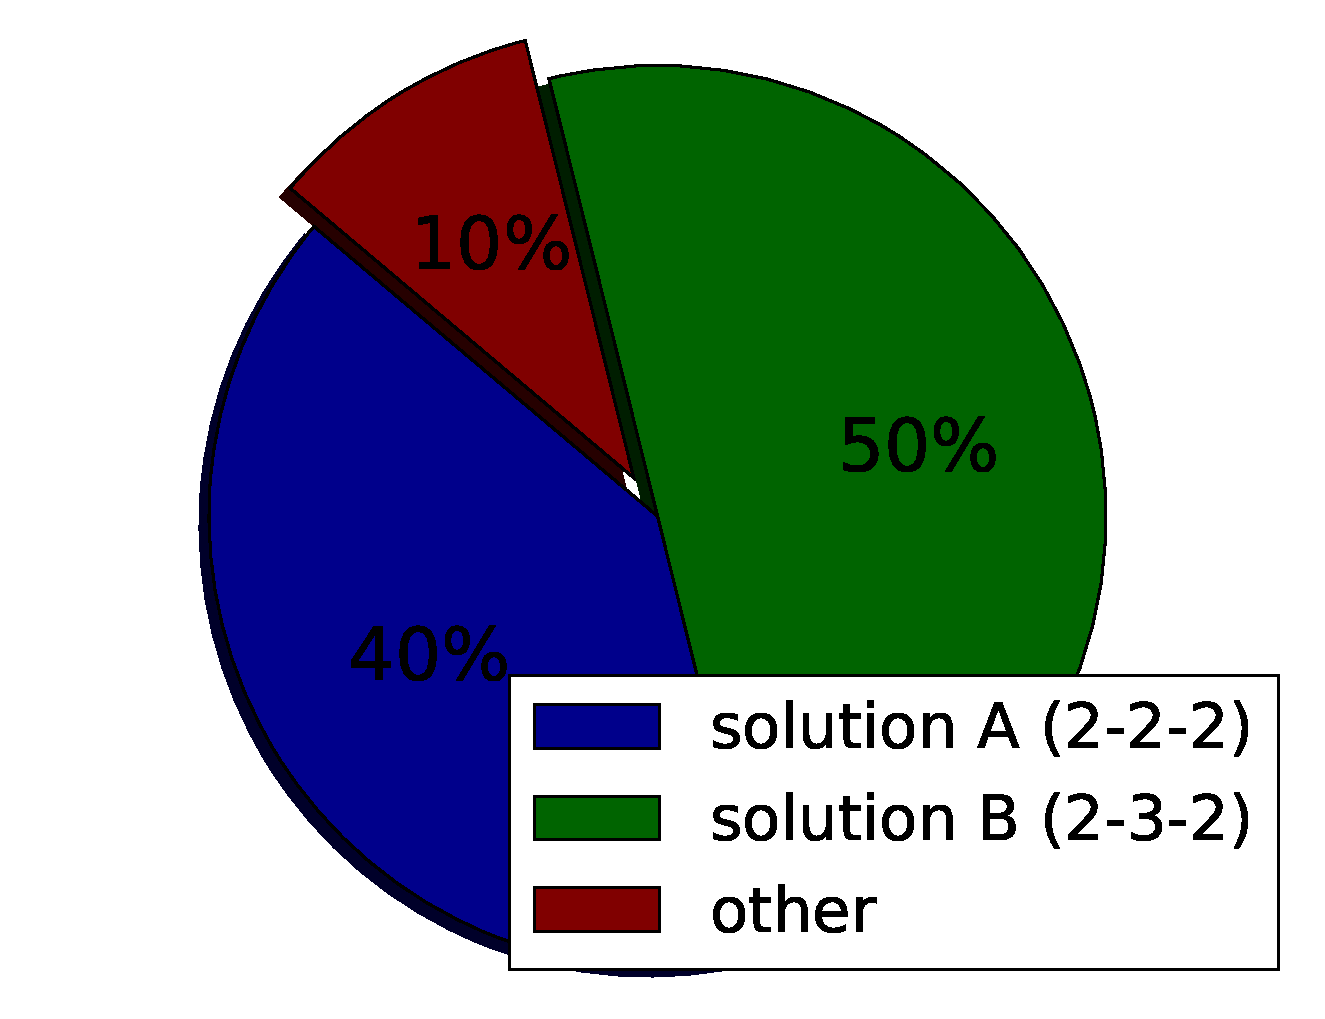
\includegraphics[height=4cm]{pruning_result_pie_xor.eps}
  \caption{Network structure after pruning (100 observations).}
  \label{fig:examples:pie_xor}
\end{subfigure}
\begin{subfigure}{.4\textwidth}
  \centering
  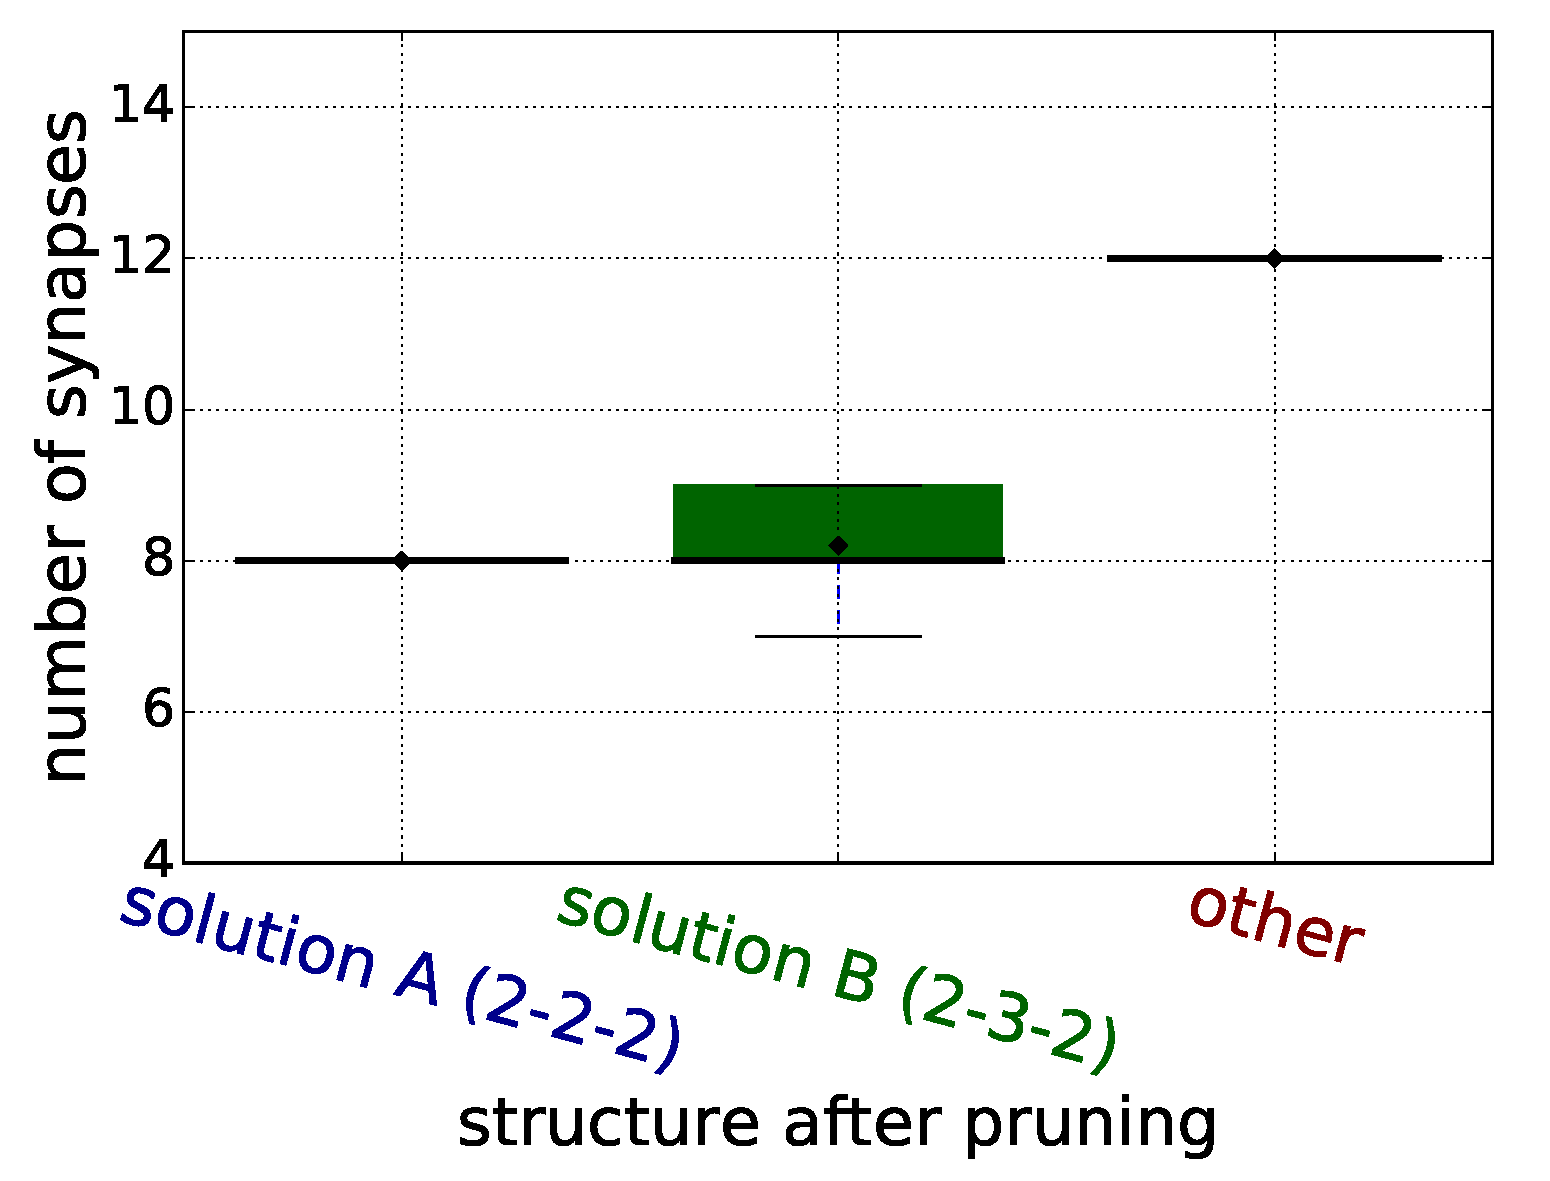
\includegraphics[height=4cm]{pruning_result_synapses_xor.eps}
  \caption{Number of synapses after pruning (100 observations).}
  \label{fig:examples:result_synapses_xor}
\end{subfigure}
\caption{Pruning results for XOR dataset.}
\label{fig:examples:pruning_result_xor}
\end{figure}

\section{2D-problem: Unbalanced Feature Information} \label{sec:dataset_unbfea}
This example is adopted from \citep{karnin}. The problem is again two-dimensional having two non-overlapping classes as depicted in \cref{fig:examples:dataset_unbfea}. The samples are uniformly distributed in $ [-1, 1] $ x $ [-1, 1] $ and the classes are equally probable, separated by two lines in 2D space ($ x_1 = a $ and $ x_2 = b $, where $ a = 0.1 $ and $ b = \frac{2}{a+1} - 1 \approx 0.82 $). Clearly, the problem can be solved by two neurons, similarly as the previous one.

What is interesting about this two-classes layout is that feature $ x_1 $ is much more important for the global classification accuracy than feature $ x_2 $. Having $ x_1 $ information, based on \cref{fig:examples:dataset_unbfea} one could potentially classify more than $ 90\% $ of the samples. Opposite of that, we cannot say much with information from feature $ x_2 $ only. And this is something what also the pruning algorithm should find out.

\begin{figure}[H]
\centering
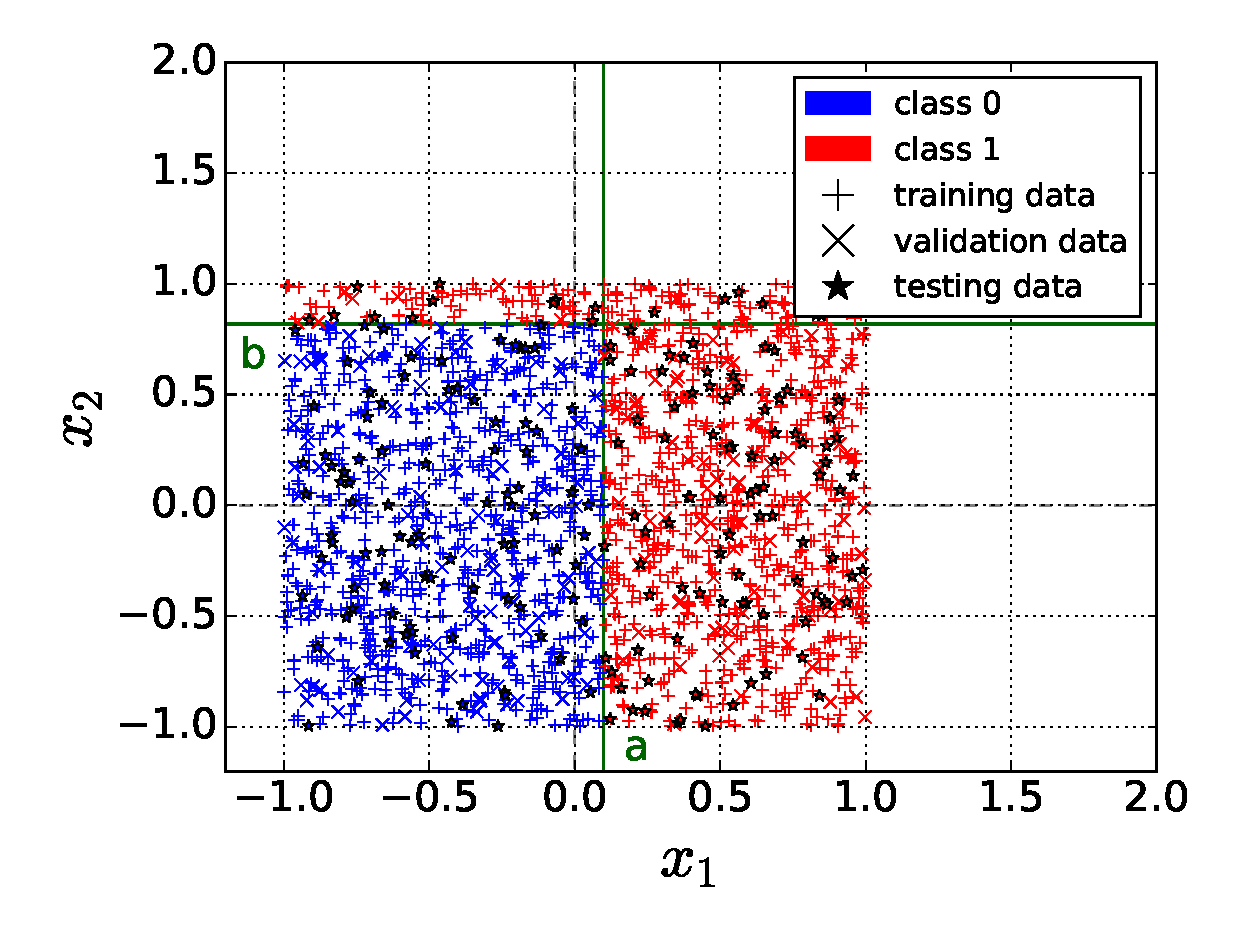
\includegraphics[width=0.85\textwidth]{dataset_unbfea.eps}
\caption{Dataset with unbalanced feature information.}
\label{fig:examples:dataset_unbfea}
\end{figure}

Hence, we focus on synapses connecting the input and hidden layer. We know the required network structure is $ [2, 2, 2] $, as two lines are needed to separate the data in 2D space. Actually, we even know the lines must be parallel to coordinate axes, which means that each of the hidden units needs one of the features only. Therefore, the first hypothesis here is that pruning of input-hidden synapses should result in one of the cases in \cref{fig:examples:unbfea_hypos}.

\begin{figure}[H]
\centering
\begin{subfigure}{.4\textwidth}
  \centering
  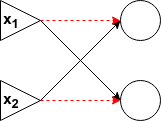
\includegraphics[height=2cm]{unbfea_hypo1}
  \caption{Pruning result 1.}
  \label{fig:examples:unbfea_hypo1}
\end{subfigure}
\begin{subfigure}{.4\textwidth}
  \centering
  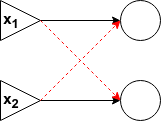
\includegraphics[height=2cm]{unbfea_hypo2}
  \caption{Pruning result 2.}
  \label{fig:examples:unbfea_hypo2}
\end{subfigure}
\caption{Expected pruning of input-hidden synapses (Unbalanced features problem).}
\label{fig:examples:unbfea_hypos}
\end{figure}

To prove this behaviour, we ran an experiment with settings in \cref{tab:examples:unbfea_settings}.

\begin{table}[H]
\centering
\scalebox{0.95}{
\begin{tabular}{|l|c|l|c|l|c|}
\hline
\multicolumn{2}{|c|}{\textit{initial network}} & \multicolumn{2}{c|}{\textit{learning parameters}} & \multicolumn{2}{c|}{\textit{pruning parameters}} \\ \hline
structure             & {[}2, 2, 2{]}          & learning rate                  & 0.7              & required accuracy             & 0.98             \\ \hline
transfer fcn          & sigmoid                & number of epochs               & 50               & retrain                       & True             \\ \hline
                      &                        & minibatch size                 & 1                & retraining epochs             & 50               \\ \hline
\end{tabular}}
\caption{Experiment settings for dataset with unbalanced feature information.}
\label{tab:examples:unbfea_settings}
\end{table}

The second hypothesis is that the synapse connected to the first feature ($ x_1 $) is more important and therefore, the other synapse (the one connected to feature $ x_2 $) will always be removed first.

\subsection*{Results: Unbalanced Feature Information}
In \cref{fig:examples:pruning_result_pie_unbfea} the first hypothesis is confirmed. The pruning of input-hidden synapses finished with the result shown in \cref{fig:examples:unbfea_hypo1} in $ 48 $ out of $ 100 $ observations and with the result in \cref{fig:examples:unbfea_hypo2} in $ 44\% $ of the cases.

\begin{figure}[H]
\centering
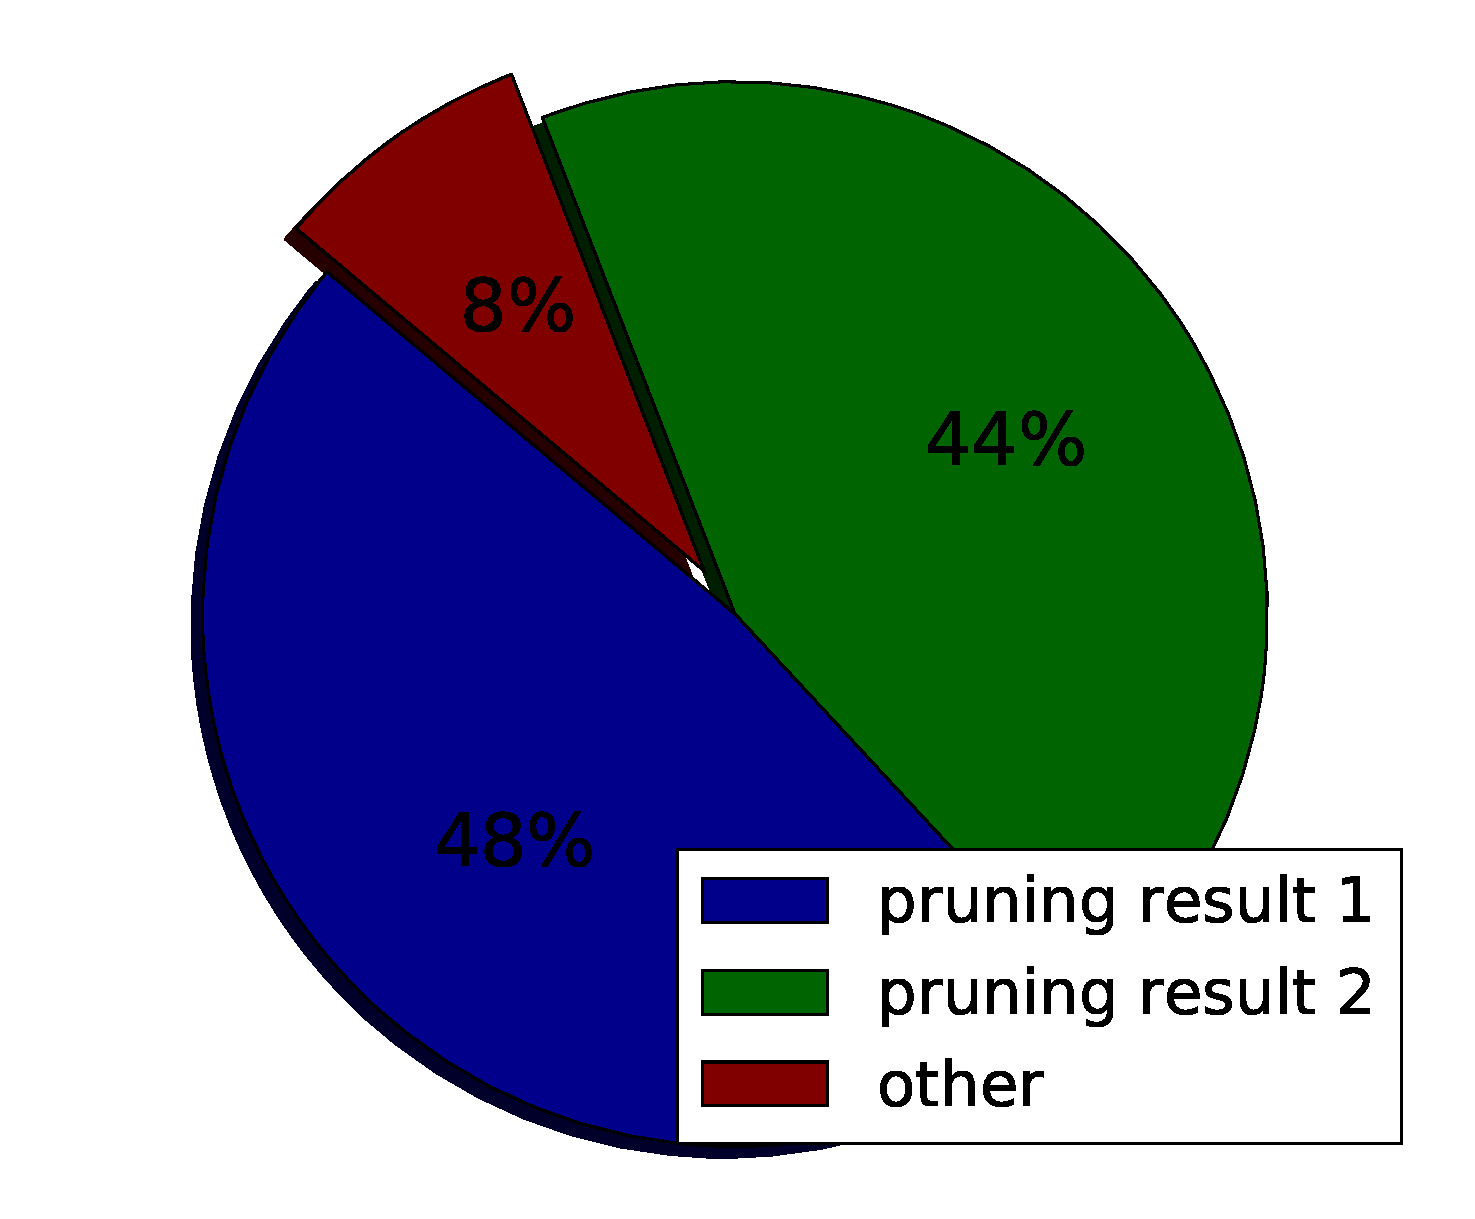
\includegraphics[width=0.5\textwidth]{pruning_result_pie_unbfea.eps}
\caption{Results of pruning (see \cref{fig:examples:unbfea_hypos}) in input-hidden layer (100 observations).}
\label{fig:examples:pruning_result_pie_unbfea}
\end{figure}

In other words, with a probability of $ 92\% $ the algorithm is able to find the axes-parallel lines and reveals that each of the lines needs information from one feature only. In the remaining $ 8\% $ of the cases the pruning resulted with more than two input-hidden synapses.

The second hypothesis is confirmed in \cref{fig:examples:unbfea_synapse_weight_change}. As we can see, the coefficient of synapses's significance was always (100 observations) greater for the synapse coming from feature $ x_1 $ than for the synapse connected to $ x_2 $. By definition (see [PA]), the pruning method eliminates the synapses with low coefficients first, therefore information coming from feature $ x_1 $ would live longer in the network than $ x_2 $ information.

This result can be explained for such simple example. Assuming $ w_{r1} $ to be the weight of synapse connecting the $ x_1 $ feature and $ r^{th} $ hidden neuron (with bias $ b_r$) and $ w_{s2} $ the weight of synapse coming from feature $ x_2 $ to $ s^{th} $ hidden neuron (with bias $ b_s $), then by neuron definition \citep{article:perceptron} we created two lines, perpendicular one to each other, as follows.
\begin{align}
w_{r1} \cdot x_1 + 0 \cdot x_2 &= b_r \\
x_1 &= \frac{b_r}{w_{r1}} \\
0 \cdot x_1 + w_{s2} \cdot x_2 &= b_s \\
x_2 &= \frac{b_s}{w_{s2}}
\end{align}

The feature vectors are normalised (described in \cref{chap:methods}) and in \cref{fig:examples:dataset_unbfea} we see that $ |a| < |b| $, hence we want:
\begin{align}
|\frac{b_r}{w_{r1}}| &< |\frac{b_s}{w_{s2}}| \\
|w_{r1}| &> |w_{s2}|
\end{align}

Out of this we expect a weight magnitude to be greater the more important the corresponding synapse is.

\begin{figure}[H]
\centering
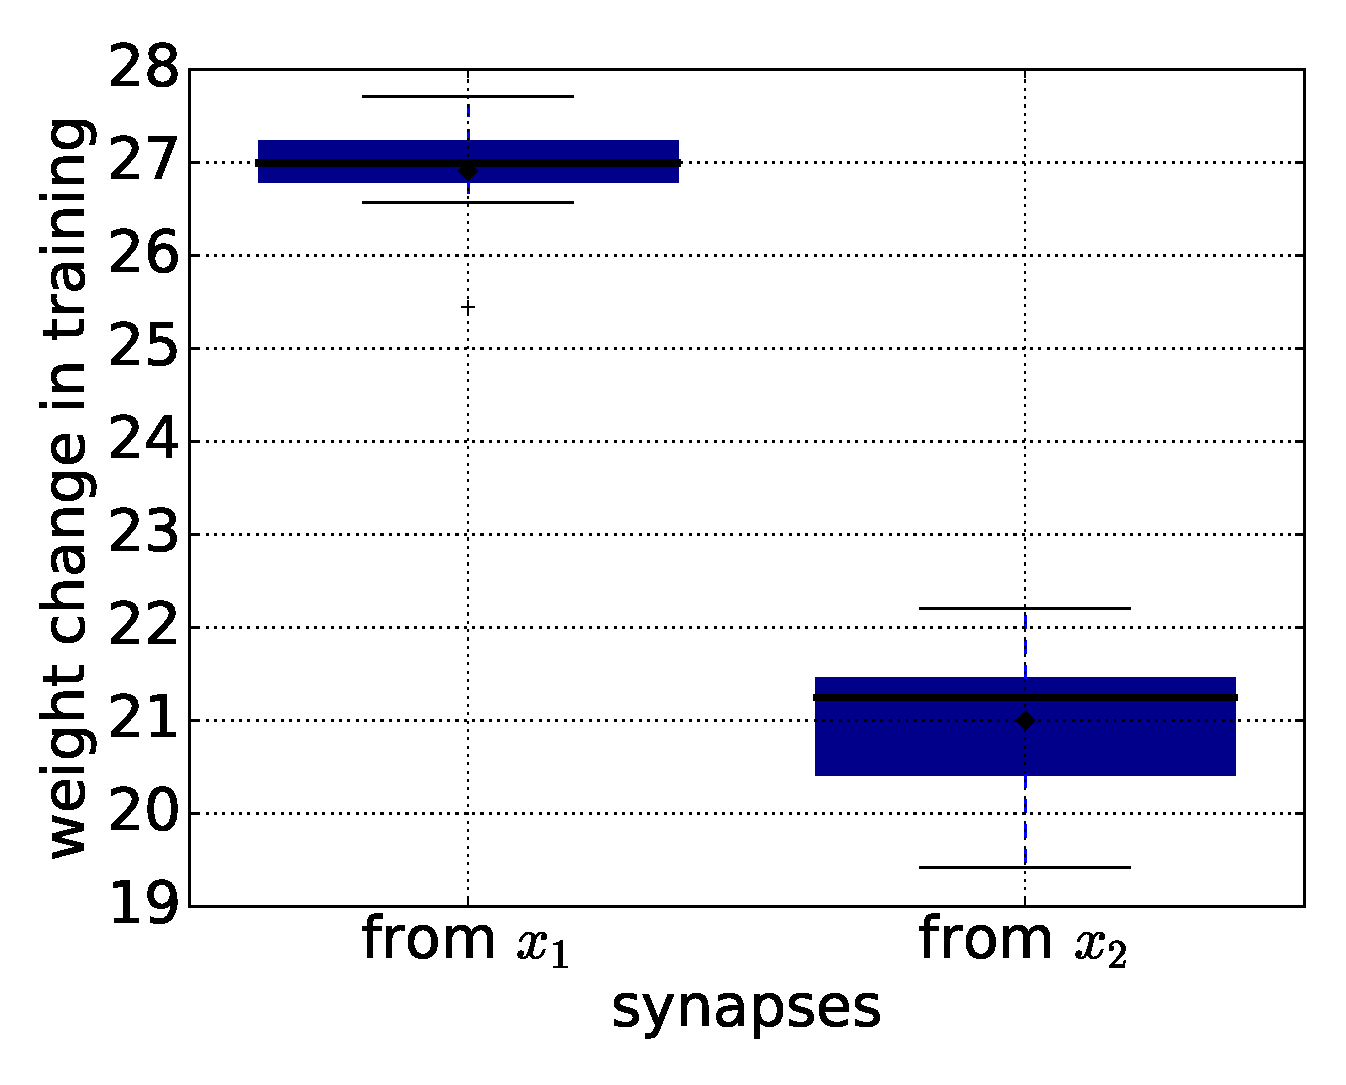
\includegraphics[width=0.75\textwidth]{unbfea_synapse_weight_change.eps}
\caption{Weight change in training for the remaining synapses in the input-hidden layer (100 observations).}
\label{fig:examples:unbfea_synapse_weight_change}
\end{figure}

However, as we do not use a weight decay (see the learning approach in \cref{chap:methods}), in general the more epochs we learn the greater the weight magnitudes are. Therefore small initial weight values does not affect the result significantly and so we can state:

\begin{equation}
|w_{ji}| \approx |w_{ji} - w0_{ji}|
\end{equation}

where $ w0_{ji} \in [0, 1] $ is the initial value of weight $ w_{ji} $. Summing it up we can say that the \textit{kitt} measure [ref] based on weight change is equally good as the magnitude measure assuming enough training epochs (e.g. 50).

\section{The Rule-plus-Exception Problem} \label{sec:dataset_rpe}
This four-dimensional problem is originally adopted from \citep{mozer_smolensky} and is also used in \citep{karnin}. The task is to learn another Boolean function: $ AB+\overline{ABCD} $. A single function output should be on (i.e. equals 1) when both $ A $ and $ B $ are on, which is the \textit{rule}, and it should also be on when the \textit{exception} $ \overline{ABCD} $ occurs.

Clearly, the \textit{rule} occurs more often than the \textit{exception}, therefore the samples corresponding with the \textit{rule} should be more important for the global classification accuracy. The hypothesis is that the pruning method will reveal the part of network, which deals with the \textit{exception}, to be eliminated first - before the part of network dealing with the \textit{rule}.

To test this example, a dataset of $ 10000 $ samples was generated. Each sample consists of four features: $ [a, b, c, d] $. Each of these features (for every sample) was randomly set to be \textit{on} ($ 1 $) or \textit{off} ($ 0 $). Then, whenever the \textit{rule} occured ($ a = 1 \wedge b = 1 $), the sample was assigned to class $ 1 $ (as a \textit{rule} sample). If the \textit{exception} occured ($ a = 0 \wedge b = 0 \wedge c = 0 \wedge d = 0 $), the sample was also labeled as $ 1 $ (as an \textit{exception} sample). Otherwise, the sample was assigned to class $ 0 $. Thereby the generated dataset consisted of:

\begin{itemize}
\item $ 2511 $ \textit{rule} samples (class $ 1 $);
\item $ 649 $ \textit{exception} samples (class $ 1 $);
\item $ 6840 $ samples in class $ 0 $.
\end{itemize}

The function is expected to be learned by two hidden neurons, one dealing with the \textit{rule} and the other one with the \textit{exception}. We focus on input-hidden layer again. Two possibilities of expected pruning result are shown in \cref{fig:examples:rpe_hypos}.

\begin{figure}[H]
\centering
\begin{subfigure}{.4\textwidth}
  \centering
  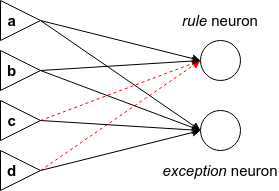
\includegraphics[height=3.5cm]{rpe_hypo1}
  \caption{Pruning result 1.}
  \label{fig:examples:rpe_hypo1}
\end{subfigure}
\begin{subfigure}{.4\textwidth}
  \centering
  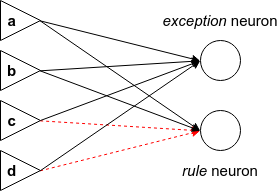
\includegraphics[height=3.5cm]{rpe_hypo2}
  \caption{Pruning result 2.}
  \label{fig:examples:rpe_hypo2}
\end{subfigure}
\caption{Expected pruning of input-hidden synapses (RPE problem).}
\label{fig:examples:rpe_hypos}
\end{figure}

We ran the learning-pruning procedure with the settings listed in \cref{tab:examples:rpe_settings}.

\begin{table}[H]
\centering
\scalebox{0.95}{
\begin{tabular}{|l|c|l|c|l|c|}
\hline
\multicolumn{2}{|c|}{\textit{initial network}} & \multicolumn{2}{c|}{\textit{learning parameters}} & \multicolumn{2}{c|}{\textit{pruning parameters}} \\ \hline
structure             & {[}2, 2, 2{]}          & learning rate                  & 1.0              & required accuracy             & 1.0             \\ \hline
transfer fcn          & sigmoid                & number of epochs               & 50               & retrain                       & True             \\ \hline
                      &                        & minibatch size                 & 1                & retraining epochs             & 50               \\ \hline
\end{tabular}}
\caption{Experiment settings for dataset with unbalanced feature information.}
\label{tab:examples:rpe_settings}
\end{table}

\subsection*{Results: The Rule-plus-Exception}
\cref{fig:examples:pruning_result_pie_rpe} supports the hypothesis that one hidden neuron forms the \textit{rule} and the other one the \textit{exception}. With a probability of $ 97\% $ the pruning finished with one of the structures in \cref{fig:examples:rpe_hypos}.

\begin{figure}[H]
\centering
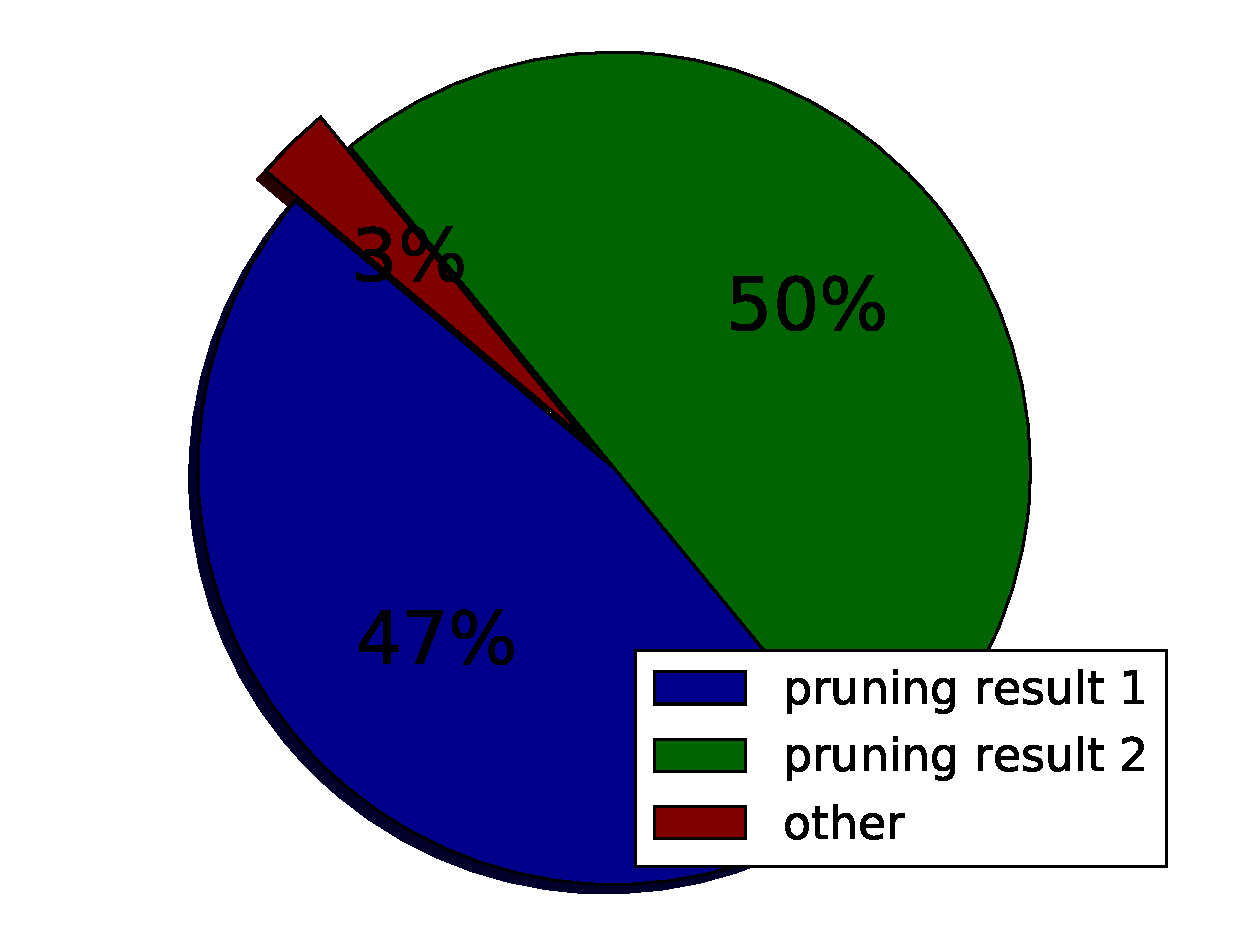
\includegraphics[width=0.5\textwidth]{pruning_result_pie_rpe.eps}
\caption{Results of pruning (see \cref{fig:examples:rpe_hypos}) in input-hidden layer (100 observations, RPE problem).}
\label{fig:examples:pruning_result_pie_rpe}
\end{figure}

The same thing is confirmed by \cref{fig:examples:pruning_result_rpe}. It shows weight changes in training (coefficients of significance) for all 8 synapses in input-hidden layer. We can see that synapses connecting the \textit{rule} neuron with feature \textit{c} ($ s_{rc}) $ and \textit{d} ($ s_{rd} $) were eliminated first (resulting in structures in \cref{fig:examples:rpe_hypos}).

\begin{figure}[H]
\centering
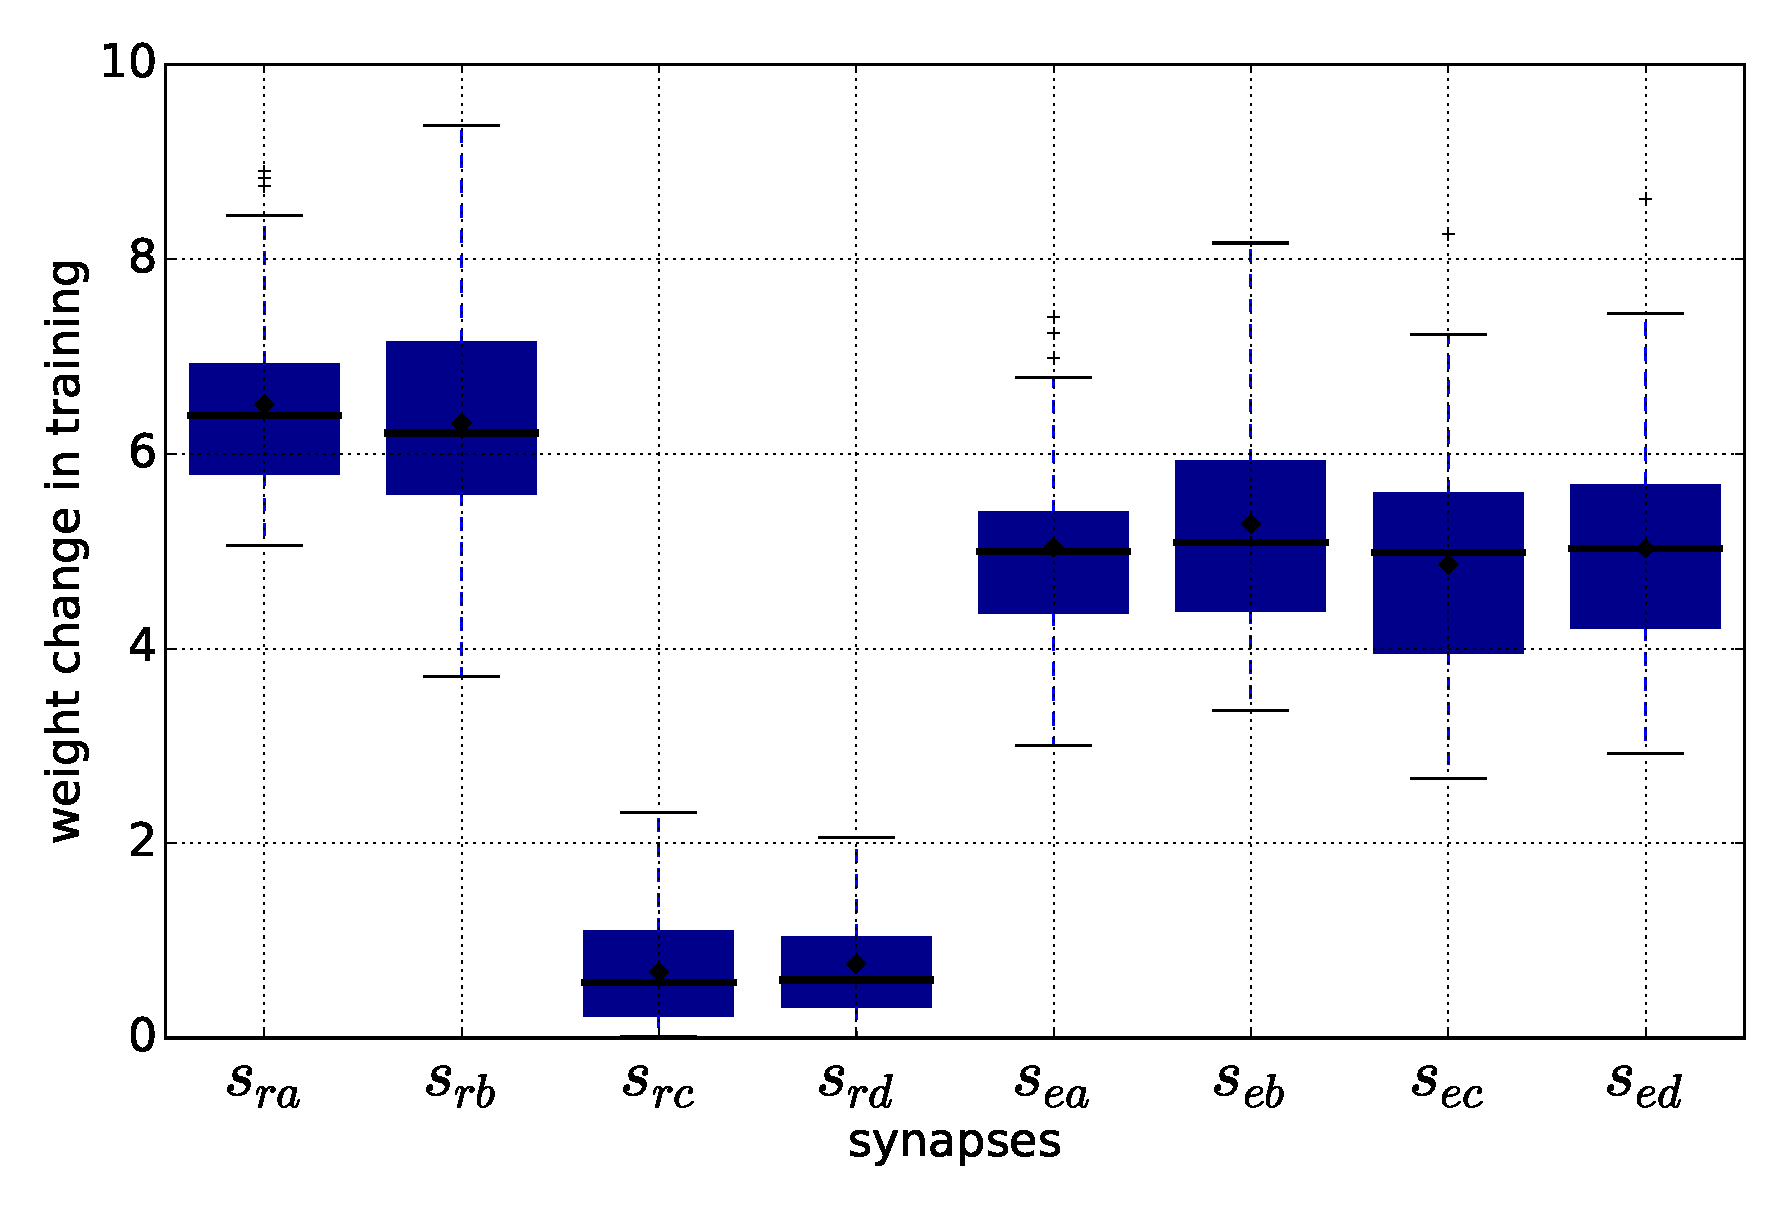
\includegraphics[width=\textwidth]{pruning_result_rpe.eps}
\caption{Weight change in training for synapses in input-hidden layer (100 observations, RPE problem).}
\label{fig:examples:pruning_result_rpe}
\end{figure}

Additionally, synapses responsible for \textit{rule} ($ s_{ra} $ and $ s_{rb} $) have greater mean significance than the synapses connected with the \textit{exception} neuron ($ s_{e*} $).

\section{The Train Problem} \label{sec:dataset_train}
The Michalski's train problem...

\begin{figure}[H]
\centering
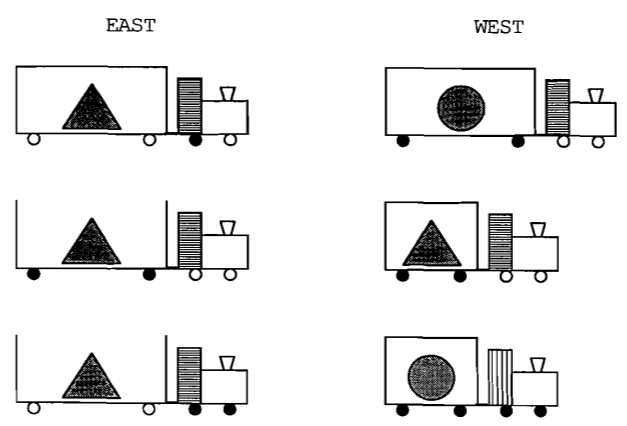
\includegraphics[width=0.7\textwidth]{train_problem}
\caption{Michalski's train problem.}
\label{fig:examples:dataset_train}
\end{figure}

\section{Handwritten digits (MNIST)} \label{sec:dataset_mnist}
MNIST data... \citep{online:mnist}

\section{Phonemes (Speech Data)} \label{sec:dataset_phonemes}
PHONES data...
